\section{Results}
\label{sec:results}
In this section the experiments results are compared with the predictions. Additionally some relevant plots are explained to show useful insights. In all cases the tests results are coherent with the predictions (which is an upper bound). In the Ethernet scenario the values are almost equal to predictions while in the Both Wi-Fi scenario and in the Mixed scenario the test results are lower then the predictions mostly due to throughput variations over a wireless link.

\subsection{TCP}
The predictions are compared with the actual results for each scenario in Table \ref{tab:tcp_results} for TCP, and in Table \ref{tab:udp_results} for UDP. Those results were obtained using the script inserted in \ref{sec:appendix}. Results in the table are goodput values, while plots are throughput values arrived at receiver (throughput and goodput plots have the same trend, they are almost equivalent graphically). These plots are taken from the receiver side.\\

\vspace{-13pt}

\begin{table}[H]
\resizebox{7cm}{!}{
\begin{tabular}{|ll|lllll|}
\hline
\multicolumn{2}{|c|}{\multirow{2}{*}{Test}} & \multicolumn{5}{c|}{TCP: Goodput per flow (Mbps)} \\ \cline{3-7} 
\multicolumn{2}{|c|}{} & \multicolumn{1}{c|}{Prediction} & \multicolumn{1}{c|}{Average} & \multicolumn{1}{c|}{Min} & \multicolumn{1}{c|}{Max} & \multicolumn{1}{c|}{Std} \\ \hline
\multicolumn{1}{|l|}
{\multirow{2}{*}{\makecell{Both \\ Ethernet}}} & A $\rightarrow$ B & \multicolumn{1}{l|}{949} & \multicolumn{1}{l|}{940.9} & \multicolumn{1}{l|}{940} & \multicolumn{1}{l|}{941} & 0.3 \\ \cline{2-7} 
\multicolumn{1}{|l|}{} & B $\rightarrow$ A & \multicolumn{1}{l|}{949} & \multicolumn{1}{l|}{940.4} & \multicolumn{1}{l|}{938} & \multicolumn{1}{l|}{941} & 0.92 \\ \hline
\multicolumn{1}{|l|}
{\multirow{2}{*}{\makecell{Both \\Wi-Fi}}} & A $\rightarrow$ B &  \multicolumn{1}{l|}{346.8} & \multicolumn{1}{l|}{239.2} & \multicolumn{1}{l|}{210} & \multicolumn{1}{l|}{268} & 15.37 \\ \cline{2-7} 
\multicolumn{1}{|l|}{} & B $\rightarrow$ A & \multicolumn{1}{l|}{346.8} & \multicolumn{1}{l|}{201.5} & \multicolumn{1}{l|}{158} & \multicolumn{1}{l|}{240} & 25.71 \\ \hline
\multicolumn{1}{|l|}{\multirow{2}{*}{Mixed}} & A $\rightarrow$ B & \multicolumn{1}{l|}{693.6} & \multicolumn{1}{l|}{530.8} & \multicolumn{1}{l|}{470} & \multicolumn{1}{l|}{581} & 33.9 \\ \cline{2-7} 
\multicolumn{1}{|l|}{} & B $\rightarrow$ A & \multicolumn{1}{l|}{693.6} & \multicolumn{1}{l|}{595.8} & \multicolumn{1}{l|}{530} & \multicolumn{1}{l|}{639} & 31.6 \\ \hline
\end{tabular} 
}
\vspace{0.5cm}
\caption{TCP results \label{tab:tcp_results}}
\end{table}

\vspace{-20pt}

\begin{itemize}
    \item \textbf{Both Ethernet Scenario}:
        The average throughput (\ref{fig:both_eth_throughput}) for both directions (A → B and B → A) remains relatively stable after an initial increase in the first second, oscillating between 800-950 Mbps. This stability is indicated by low standard deviations (0.3 Mbps for A → B and 0.92 Mbps for B → A), suggesting a consistent performance over time. The RTT (\ref{fig:both_eth_rtt}) remains low, varying only slightly (within approximately 2.5 ms) throughout the duration of the test, indicating a reliable and stable connection, with only a few outliers (at t=1 and t=5.5).
\vspace{-20pt}
    \begin{figure}[H]
        \centering
        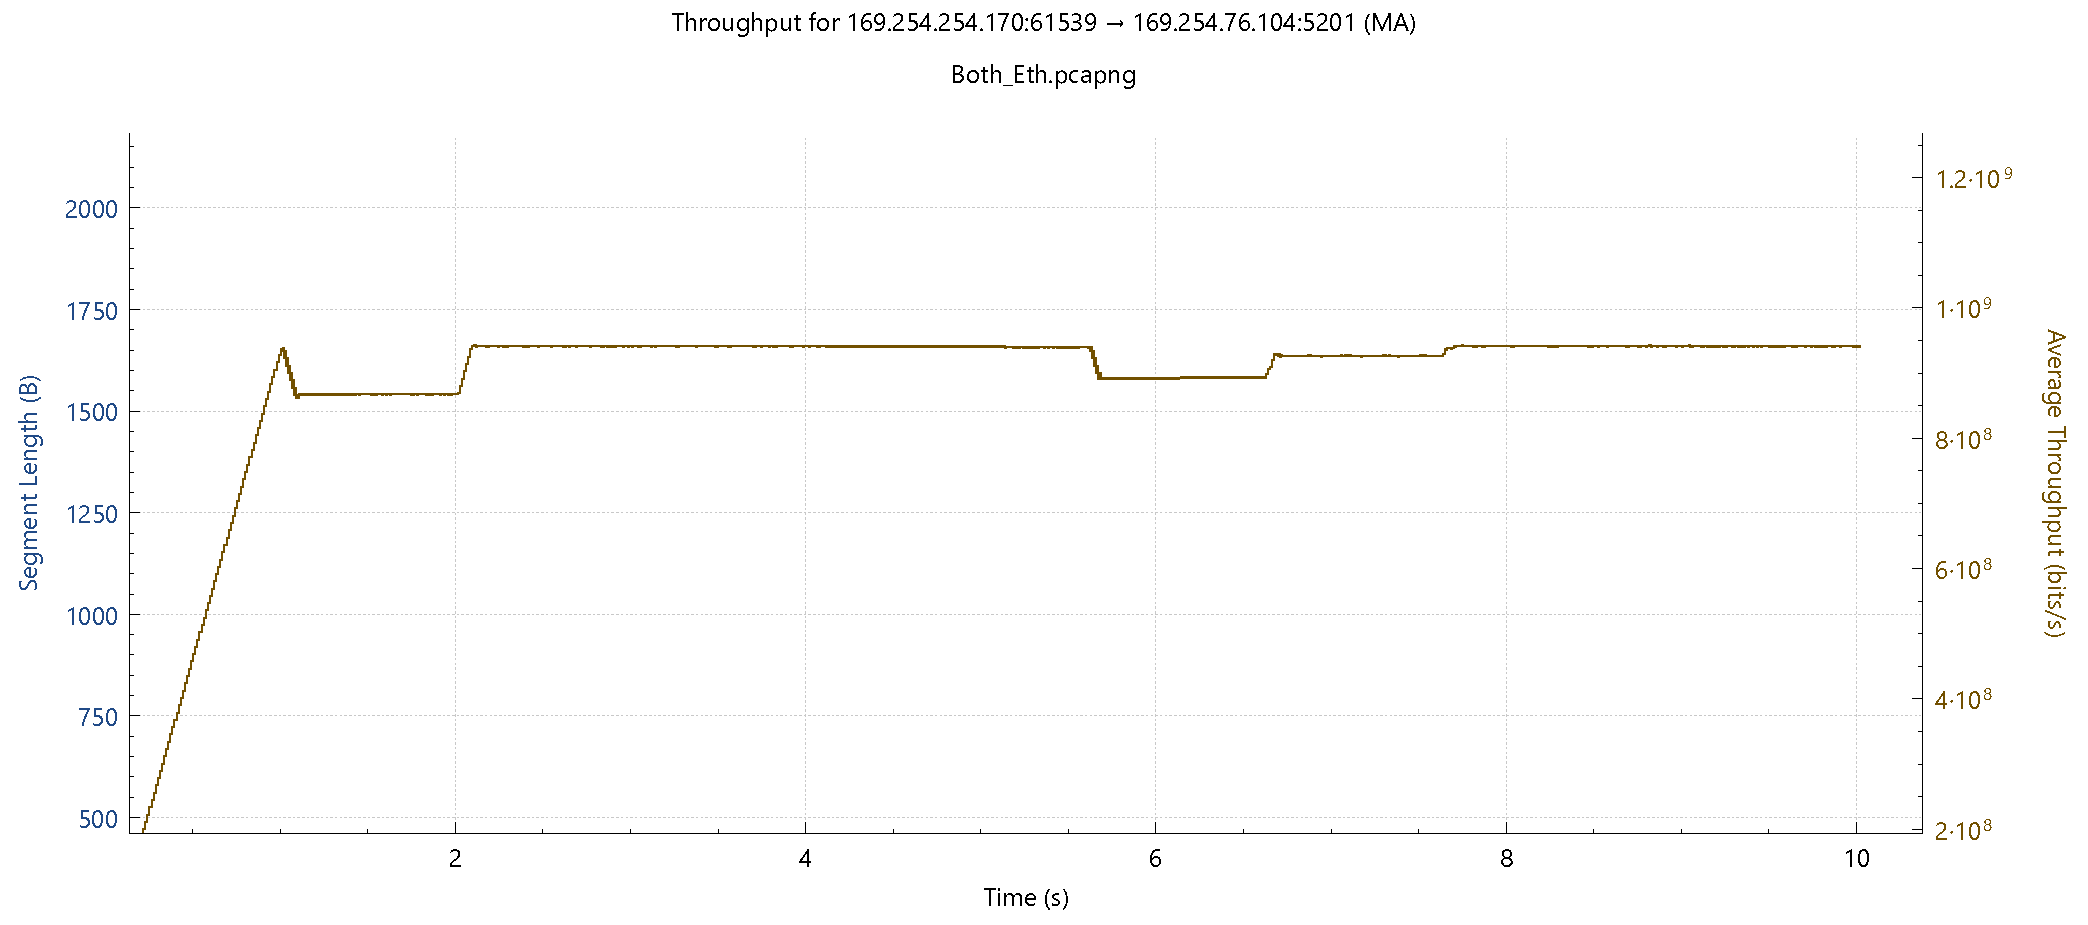
\includegraphics[width=0.4\textwidth]{images/both_eth_throughput.pdf}
        \caption{Both Ethernet Scenario Throughput}
        \label{fig:both_eth_throughput}
    \end{figure}

    \begin{figure}[H]
        \centering
        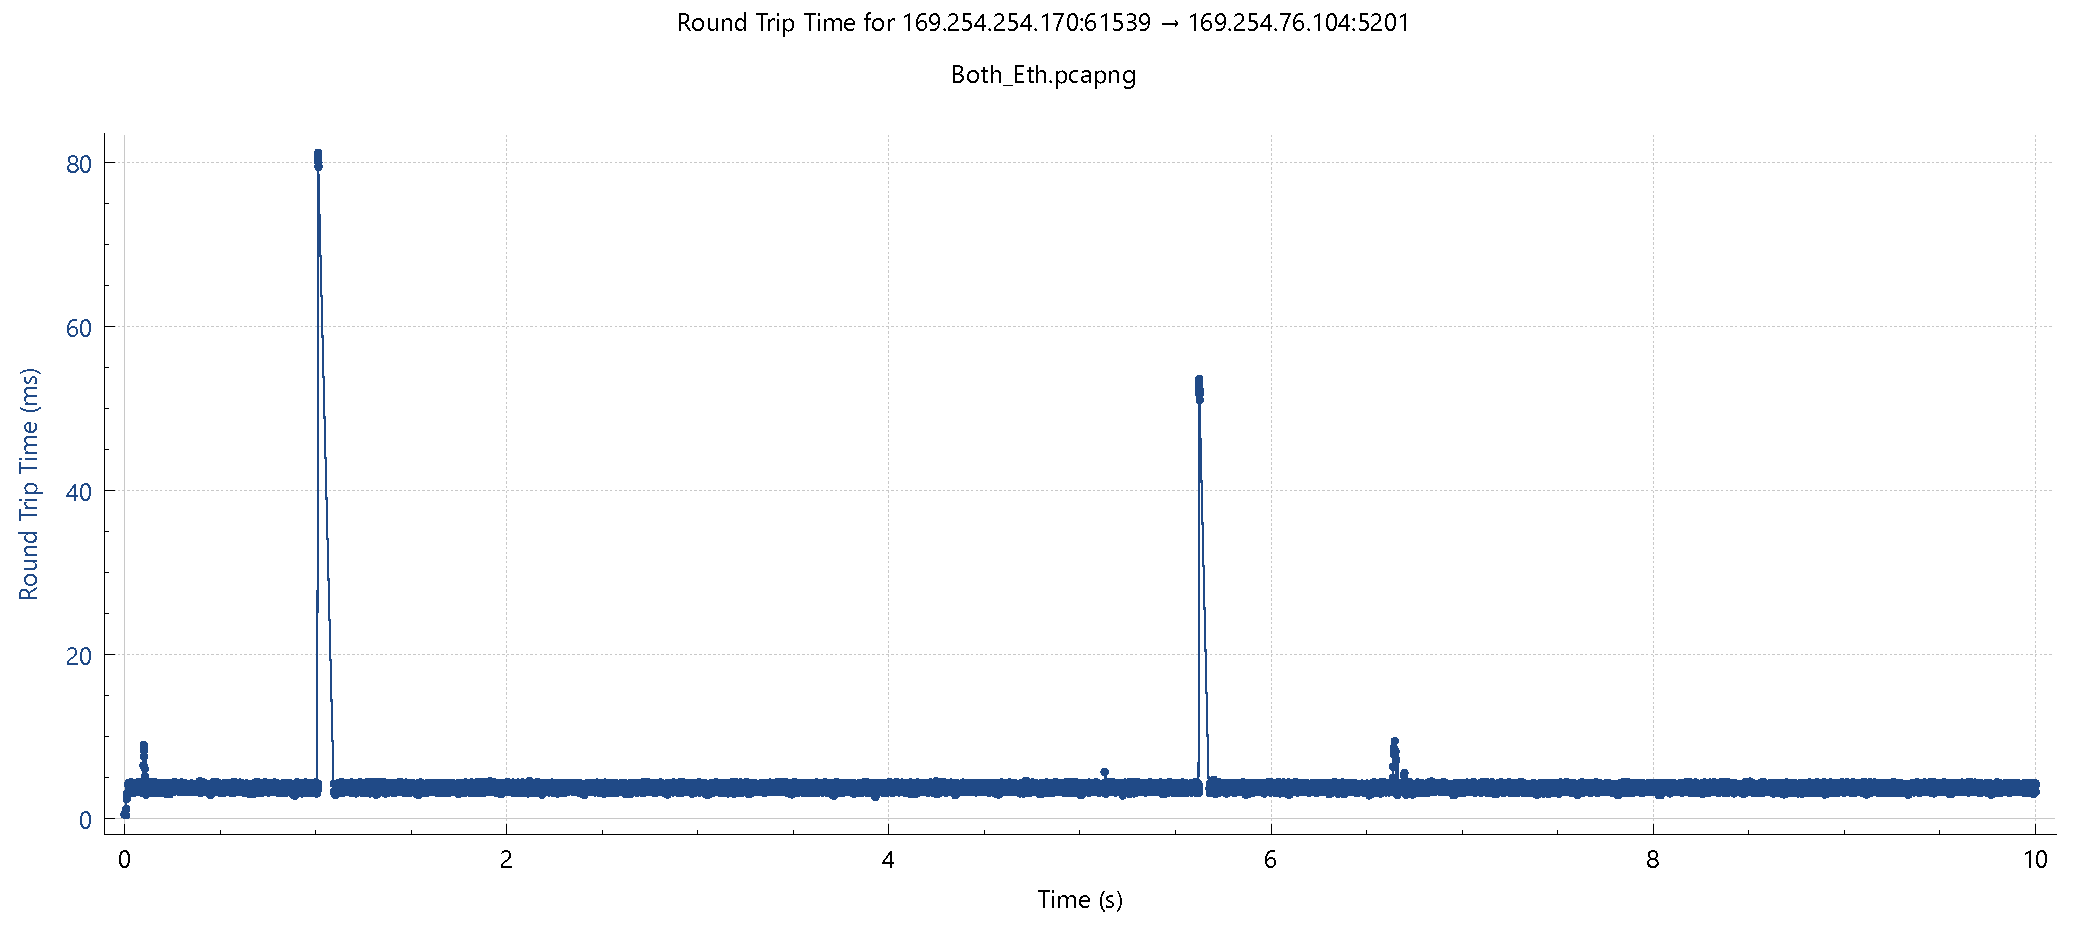
\includegraphics[width=0.4\textwidth]{images/both_eth_rtt.pdf}
        \caption{Both Ethernet Scenario RTT}
        \label{fig:both_eth_rtt}
    \end{figure}

    \item \textbf{Both Wi-Fi Scenario}:
        Unlike the Ethernet scenario, the Wi-Fi throughput (\ref{fig:both_WiFi_throughput}) exhibits more variability. It initially increases but then oscillates between approximately 225-275 Mbps after 2 seconds. This oscillation is reflected in the higher standard deviations (15.37 Mbps for A → B and 25.71 Mbps for B → A), indicating fluctuations in the connection quality caused by interference or wireless traffic. The Wi-Fi scenario exhibits the most significant variation in RTT (\ref{fig:both_wifi_rtt}), with values ranging from as low as 20 ms to as high as 155 ms, however the RTT is mainly between 20 ms and 75 ms.
        
    \begin{figure}[H]
        \centering
        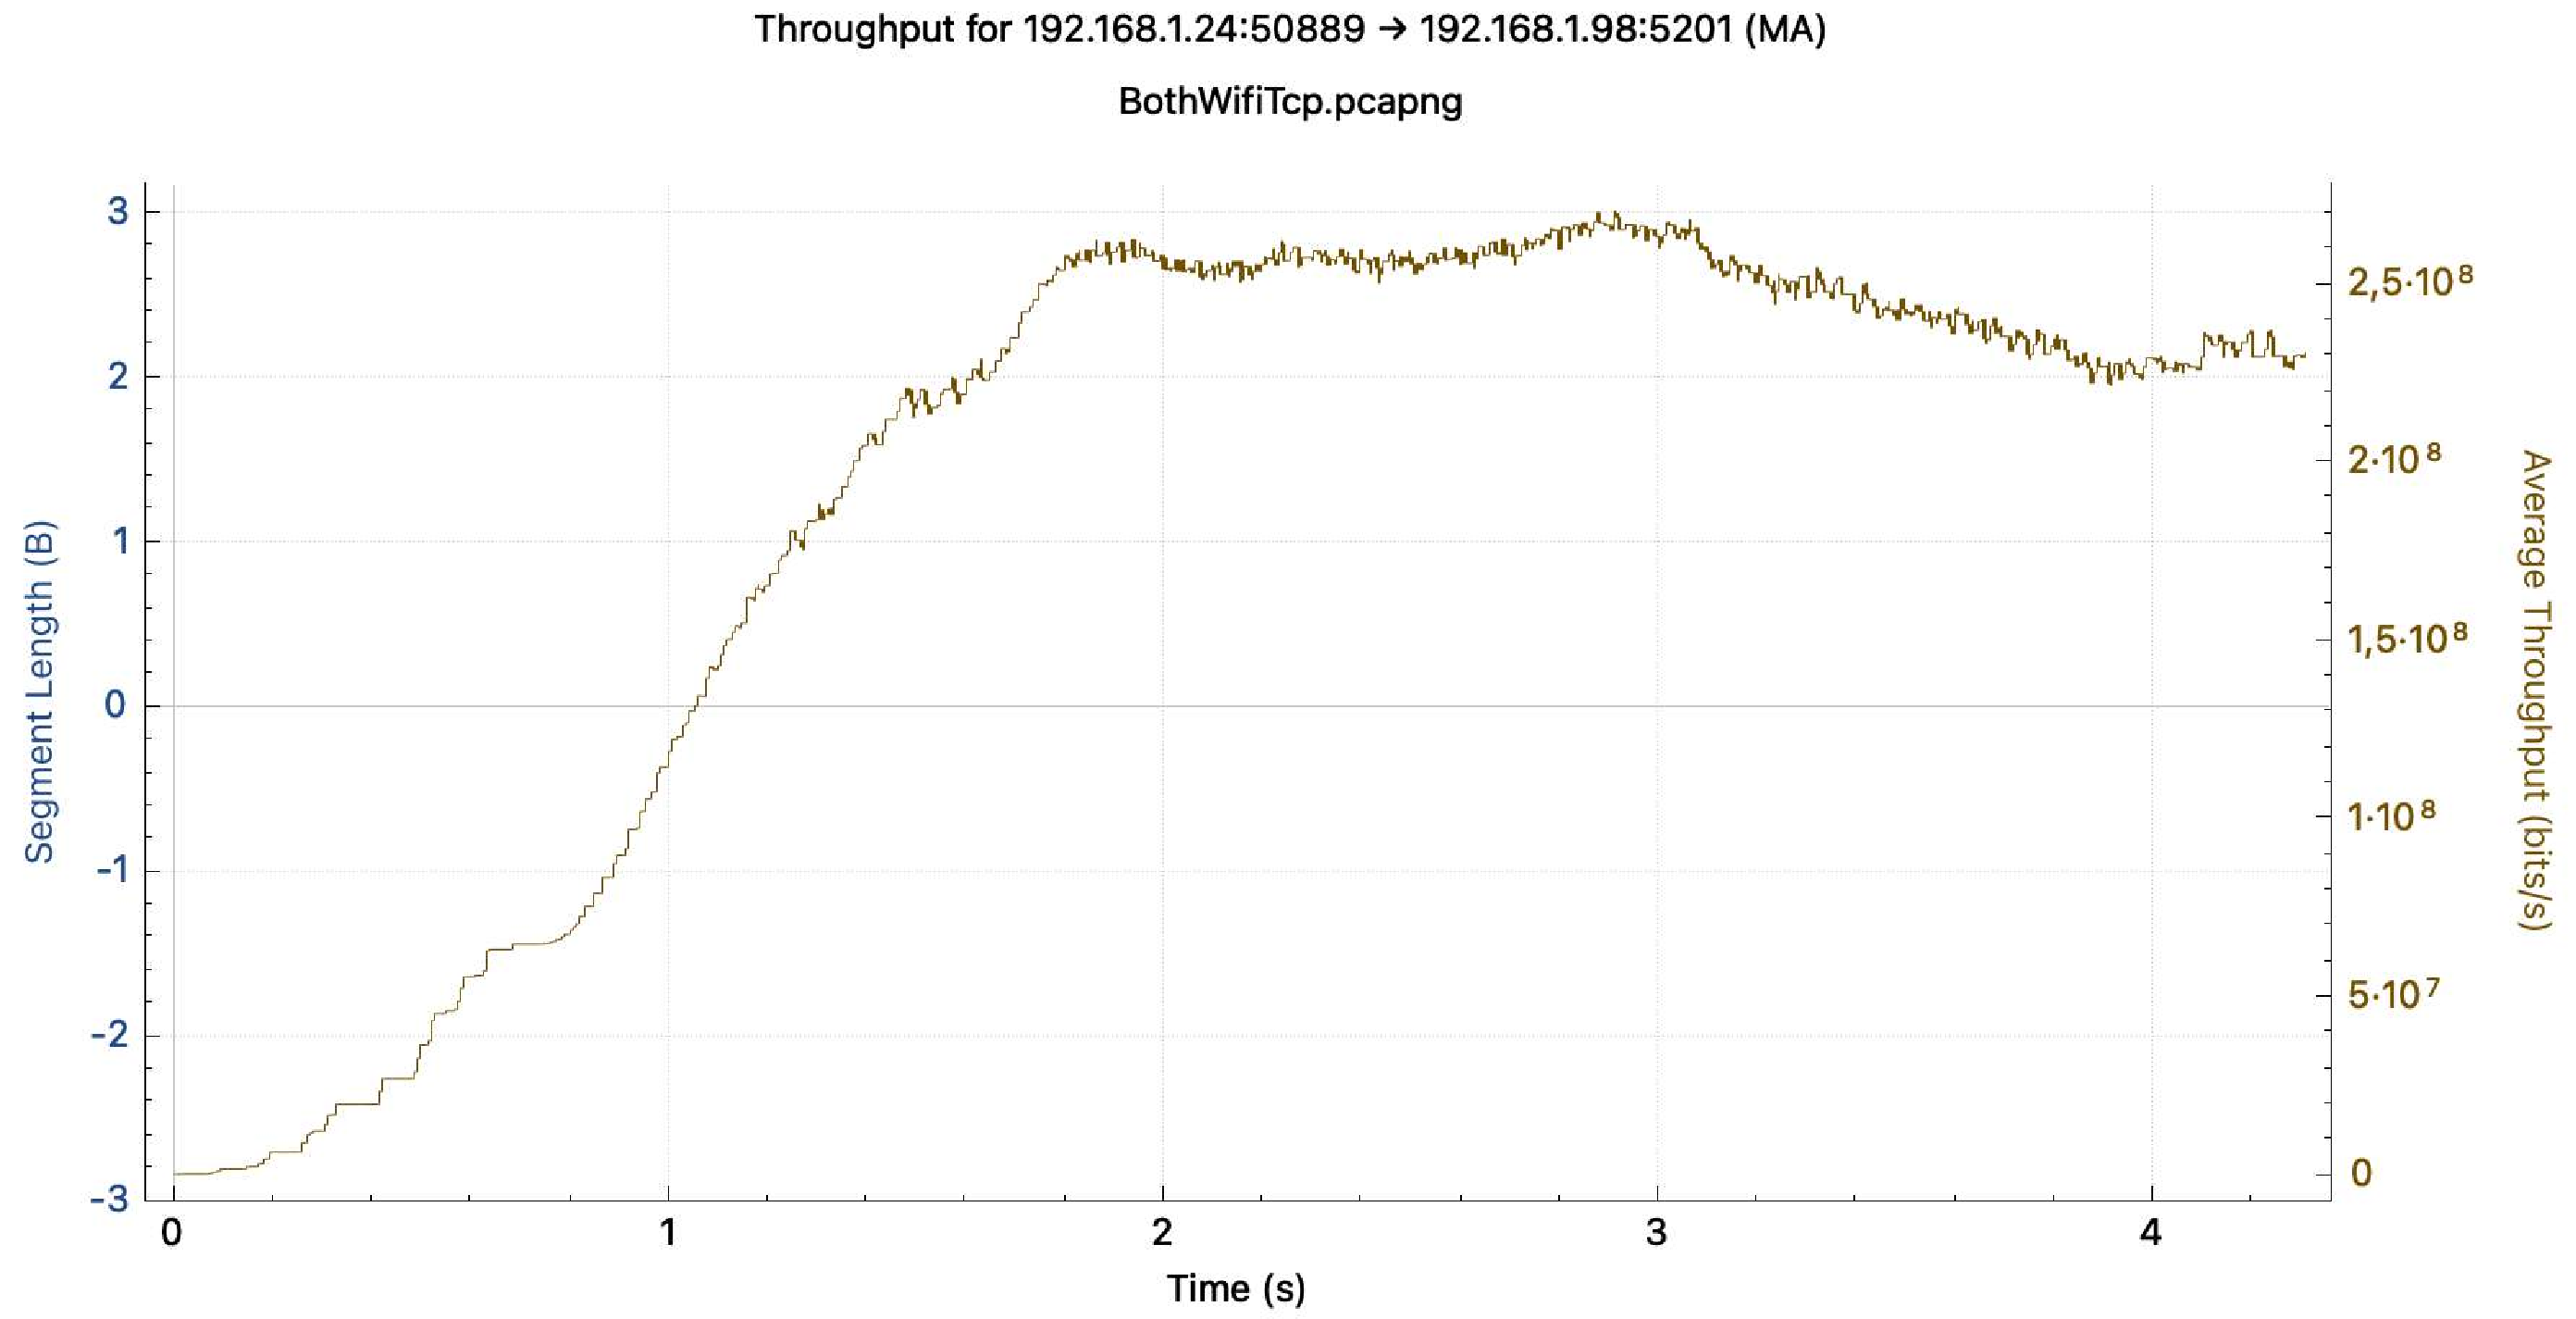
\includegraphics[width=0.4\textwidth]{images/both_wifi_throughput.pdf}
        \caption{Both Wi-Fi Scenario Throughput}
        \label{fig:both_WiFi_throughput}
    \end{figure}
    \vspace{-20pt}
    \begin{figure}[H]
        \centering
        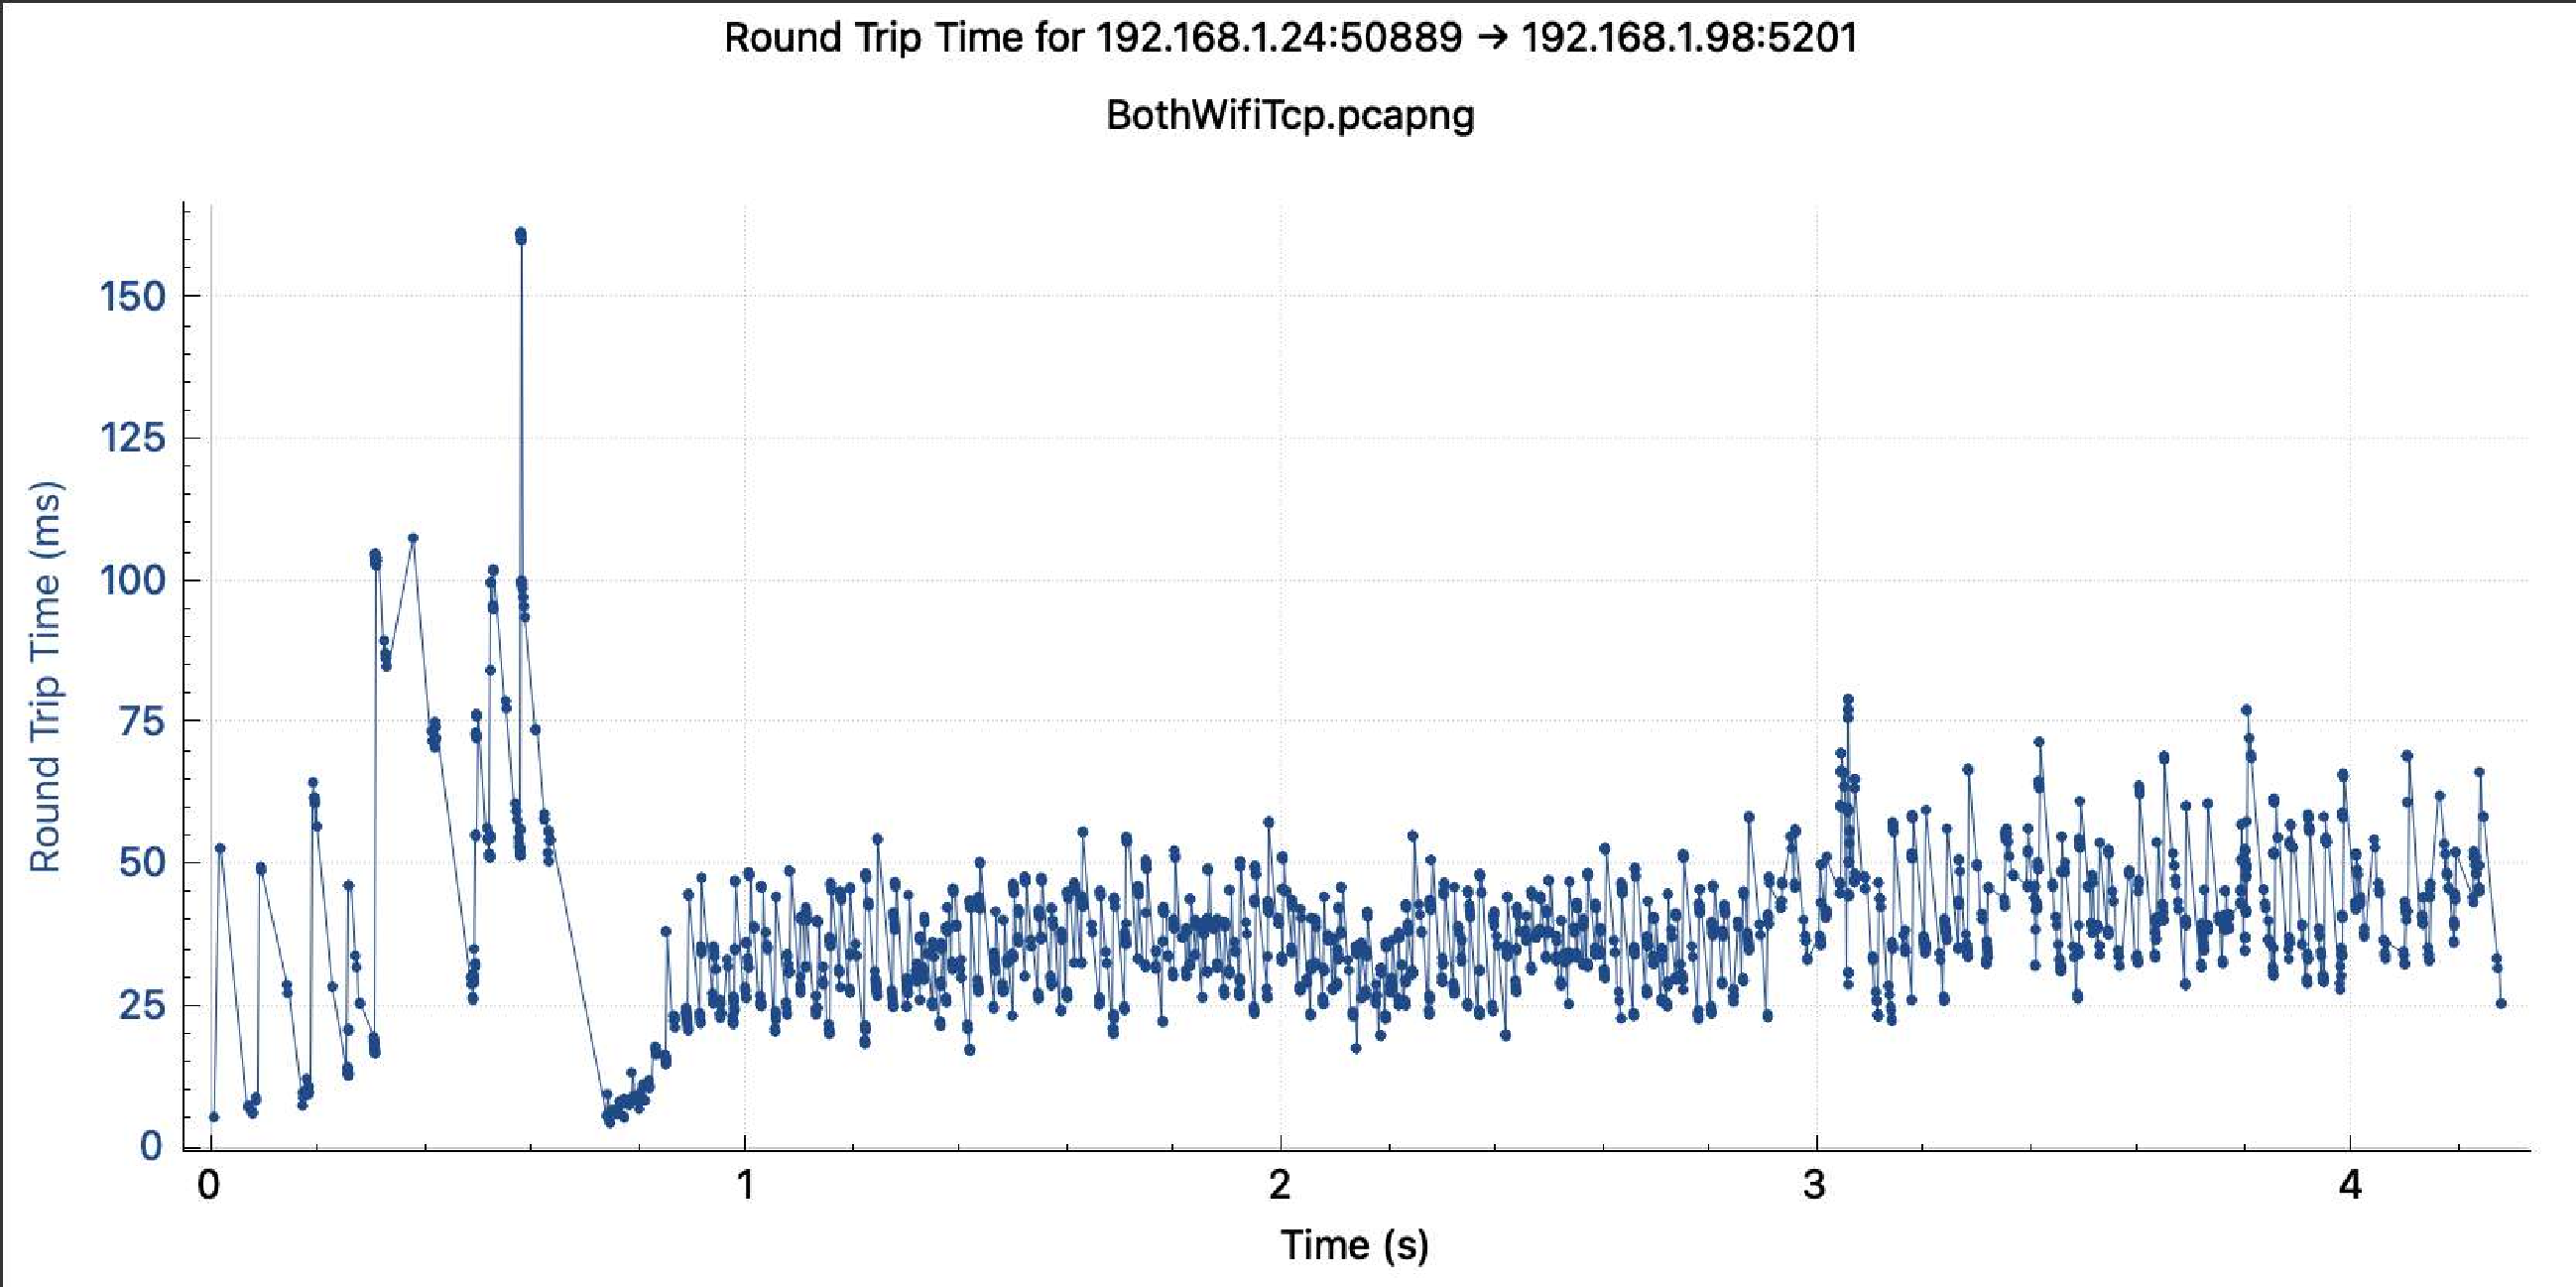
\includegraphics[width=0.4\textwidth]{images/both_wifi_rtt.pdf}
        \caption{Both Wi-Fi Scenario RTT}
        \label{fig:both_wifi_rtt}
    \end{figure}

    \item \textbf{Mixed Scenario}:
        In the mixed scenario, the throughput (\ref{fig:hybrid_throughput}) uniformly increases until reaching stability around 600-640 Mbps after the first second. The variation in throughput is relatively minor compared to the Wi-Fi scenario, and this is evident from the standard deviations (around 30 Mbps). The RTT (\ref{fig:hybrid_rtt}) oscillates less compared to the Wi-Fi scenario, as expected. The variation remains mainly within a range between 7 ms and 50 ms. This tests shows that combining Ethernet and Wi-Fi, the connection results in lower RTT values compared to the Wi-Fi to Wi-Fi setup.

    \begin{figure}[H]
        \centering
        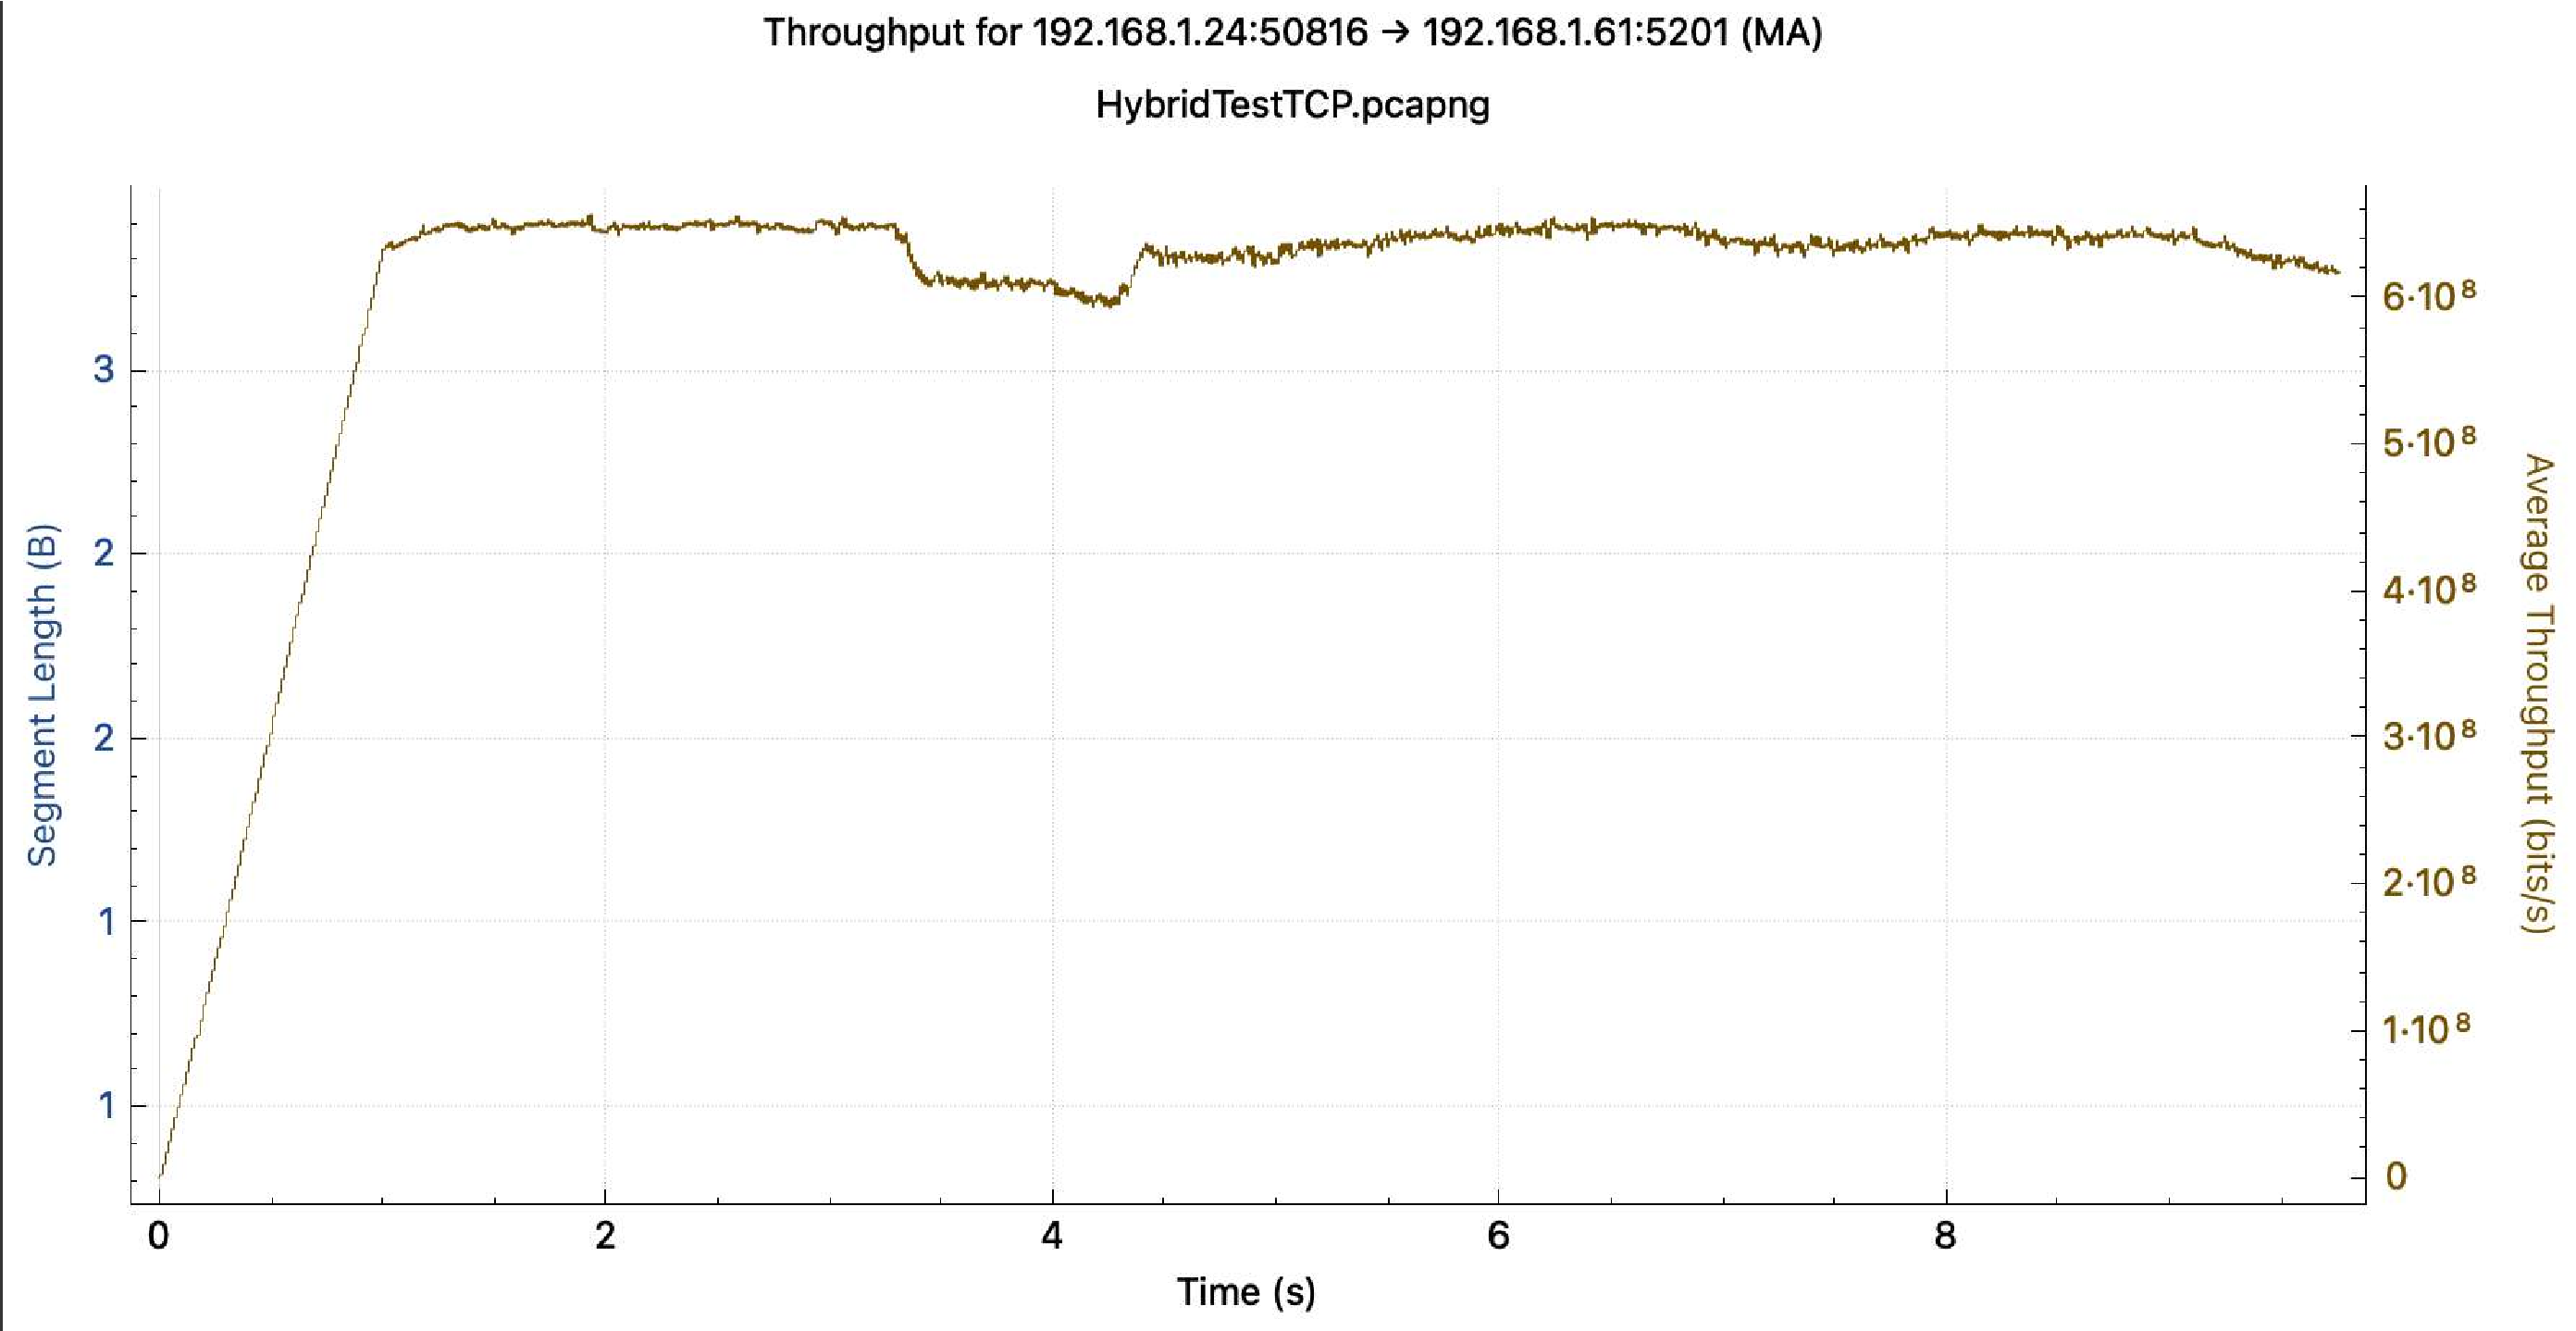
\includegraphics[width=0.4\textwidth]{images/hybrid_throughput.pdf}
        \caption{Mixed Scenario Throughput}
        \label{fig:hybrid_throughput}
    \end{figure}

    \begin{figure}[H]
        \centering
        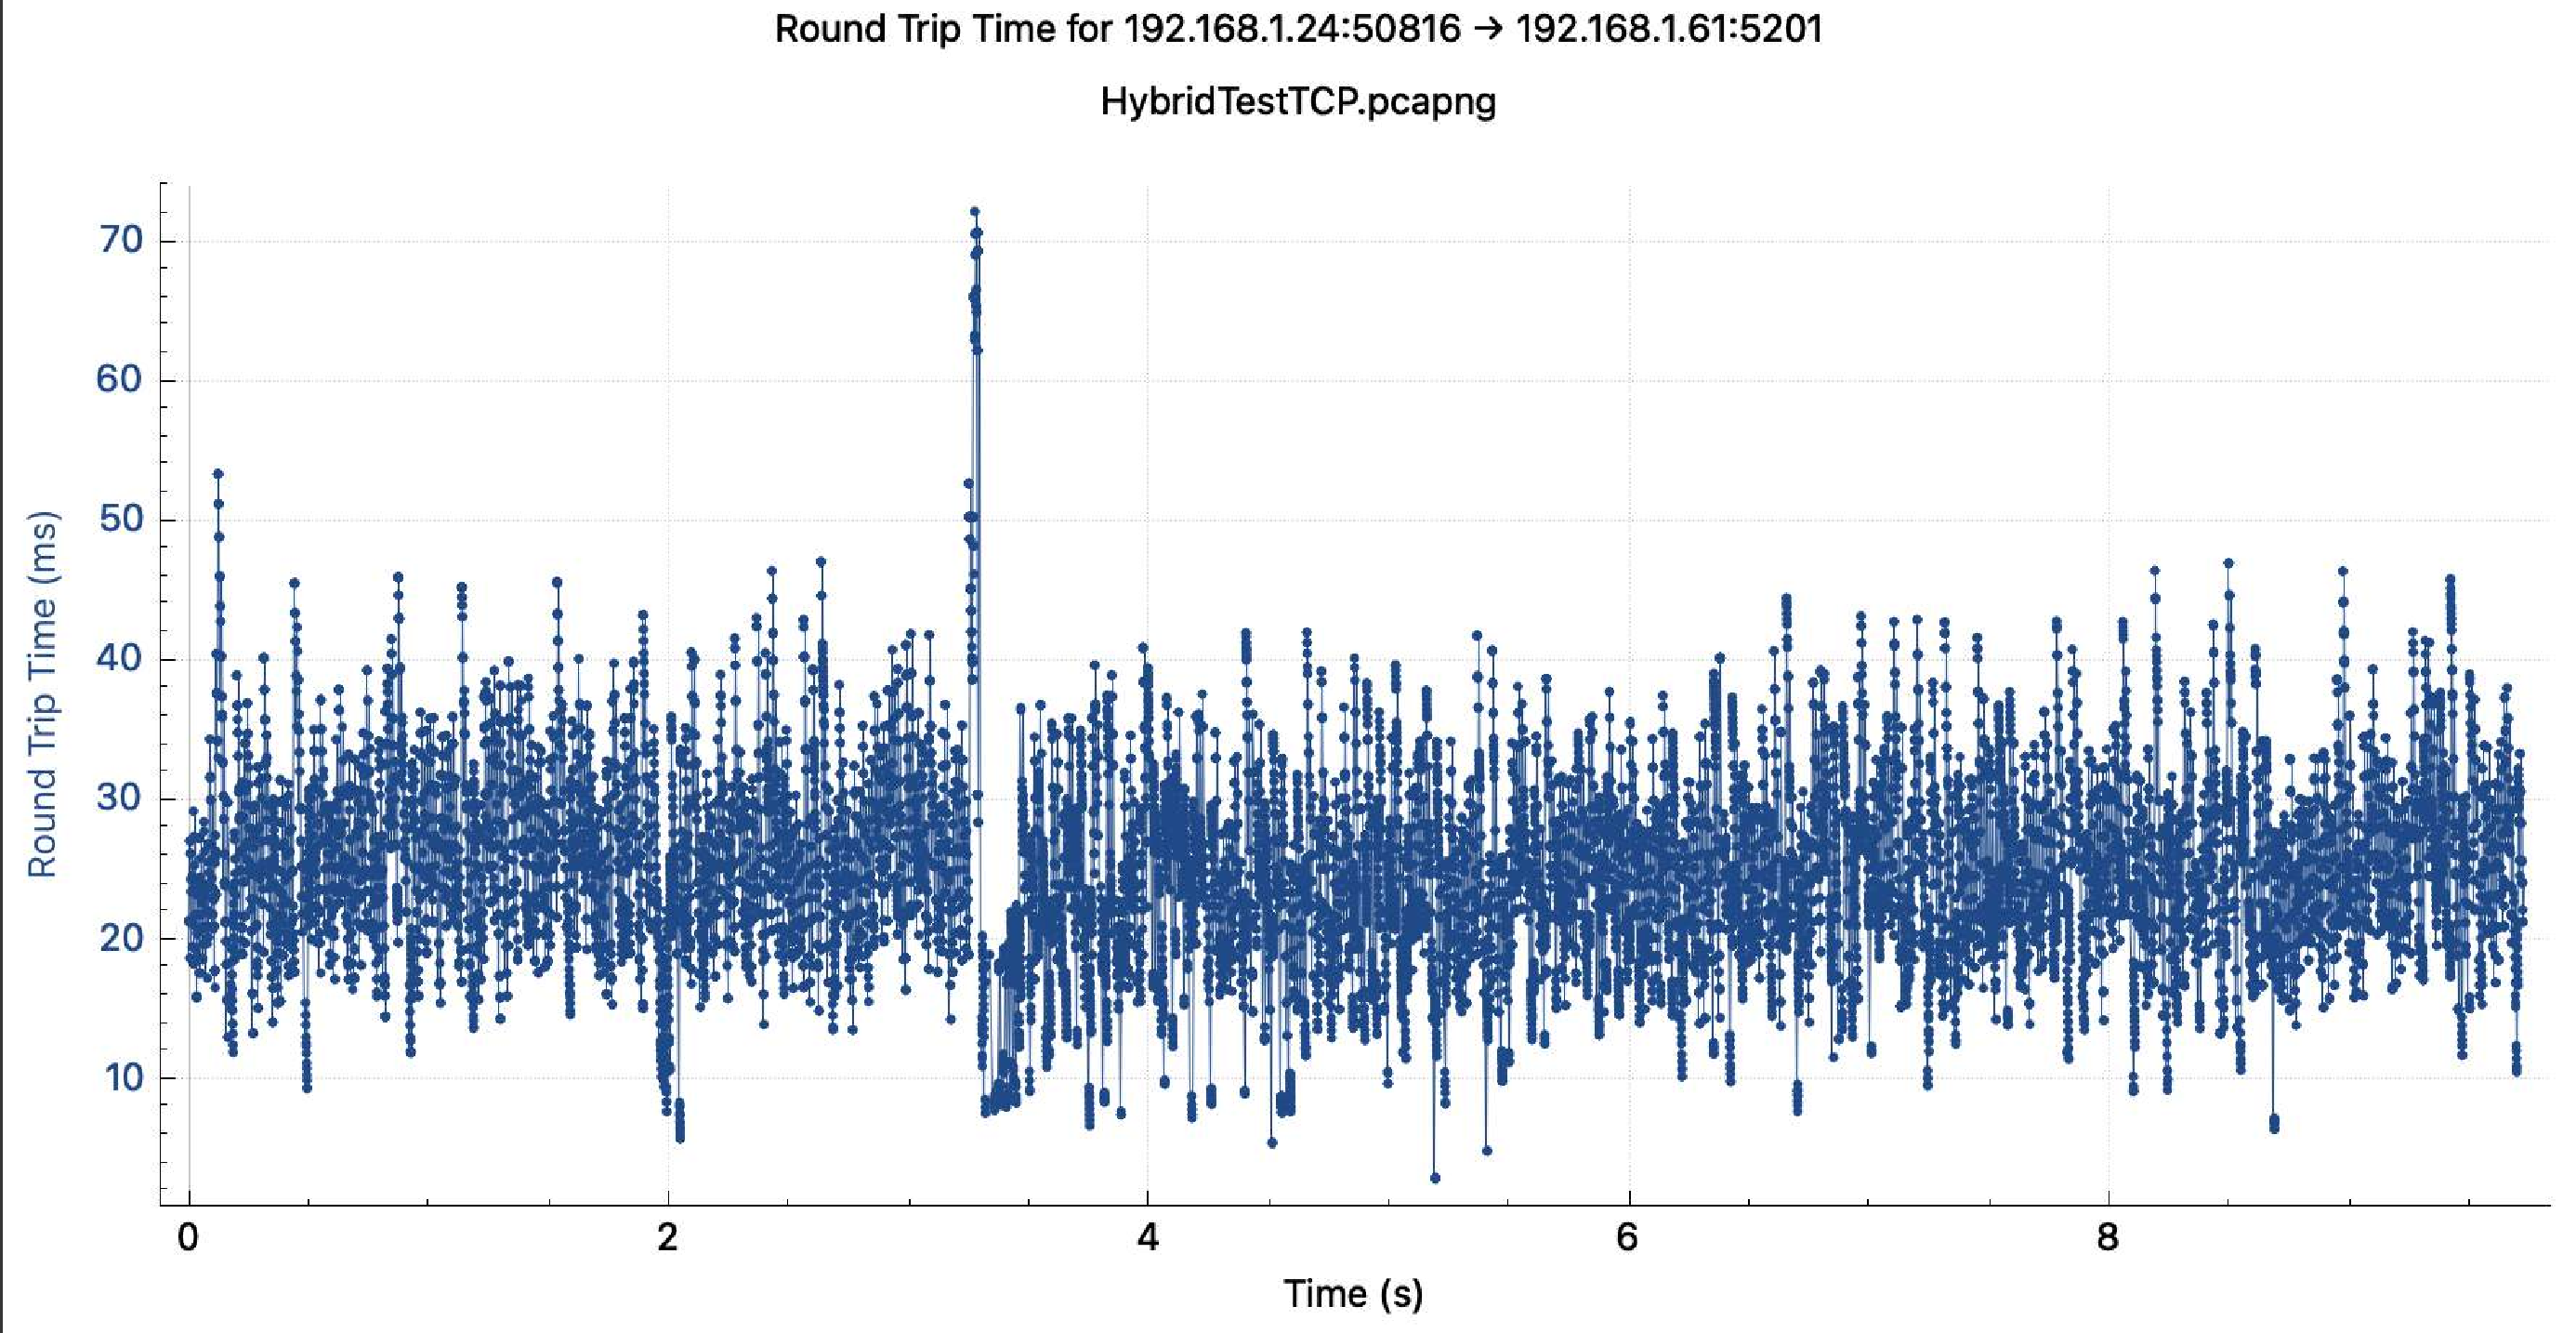
\includegraphics[width=0.4\textwidth]{images/hybrid_rtt.pdf}
        \caption{Mixed Scenario RTT}
        \label{fig:hybrid_rtt}
    \end{figure}

\end{itemize}


\subsection{UDP}

\begin{table}[H]
\resizebox{7cm}{!}{
\begin{tabular}{|ll|lllll|}
\hline
\multicolumn{2}{|c|}{\multirow{2}{*}{Test}} & \multicolumn{5}{c|}{UDP: Goodput per flow (Mbps)} \\ \cline{3-7} 
\multicolumn{2}{|c|}{} & \multicolumn{1}{c|}{Prediction} & \multicolumn{1}{c|}{Average} & \multicolumn{1}{c|}{Min} & \multicolumn{1}{c|}{Max} & \multicolumn{1}{c|}{Std} \\ \hline
\multicolumn{1}{|l|}
{\multirow{2}{*}{\makecell{Both \\ Ethernet}}} & A $\rightarrow$ B & \multicolumn{1}{l|}{957} & \multicolumn{1}{l|}{955.4} & \multicolumn{1}{l|}{953} & \multicolumn{1}{l|}{956} & 1.2 \\ \cline{2-7} 
\multicolumn{1}{|l|}{} & B $\rightarrow$ A & \multicolumn{1}{l|}{957} & \multicolumn{1}{l|}{955.2} & \multicolumn{1}{l|}{952} & \multicolumn{1}{l|}{957} & 1.47 \\ \hline
\multicolumn{1}{|l|}
{\multirow{2}{*}{\makecell{Both \\Wi-Fi}}} & A $\rightarrow$ B &  \multicolumn{1}{l|}{372.8} & \multicolumn{1}{l|}{240.9} & \multicolumn{1}{l|}{234} & \multicolumn{1}{l|}{246} & 3.3 \\ \cline{2-7} 
\multicolumn{1}{|l|}{} & B $\rightarrow$ A & \multicolumn{1}{l|}{372.8} & \multicolumn{1}{l|}{172.9} & \multicolumn{1}{l|}{108} & \multicolumn{1}{l|}{209} & 31.23 \\ \hline
\multicolumn{1}{|l|}{\multirow{2}{*}{Mixed}} & A $\rightarrow$ B & \multicolumn{1}{l|}{698.8} & \multicolumn{1}{l|}{636} & \multicolumn{1}{l|}{470} & \multicolumn{1}{l|}{581} & 33.9 \\ \cline{2-7} 
\multicolumn{1}{|l|}{} & B $\rightarrow$ A & \multicolumn{1}{l|}{698.8} & \multicolumn{1}{l|}{637.7} & \multicolumn{1}{l|}{606} & \multicolumn{1}{l|}{671} & 22.31 \\ \hline
\end{tabular} 
}
\vspace{0.5cm}
\caption{UDP results \label{tab:udp_results}}
\end{table}

\vspace{-13pt}

\begin{itemize}
    \item \textbf{Both Ethernet}:
        The average goodput for UDP in both directions over Ethernet is approximately 955 Mbps, close to the maximum value. With UDP, there is no congestion control or packet acknowledgment, so the transmitter sends packets at the maximum rate supported by the interface without guaranteeing delivery. With a both Ethernet scenario, it is possible to achieve near-maximum bandwidth utilization and basically zero \hyperlink{packet-loss}{packet loss}.

     \item \textbf{Both Wi-Fi}:
        When transmitting over Wi-Fi, the goodput drops to an average of 200 Mbps, significantly lower than Ethernet. Wi-Fi interfaces cannot immediately accept new inputs due to managing collision avoidance and Wi-Fi overhead, leading to reduced goodput compared to Ethernet. \hyperref[packet_loss]{packet loss} is more significant in this scenario, especially for transmissions from Host B to Host A. Have been observed superior performance in Wi-Fi-to-Wi-Fi and hybrid transmission scenarios when \hyperref[sec:host-a]{Host A} sends to \hyperref[sec:host-b]{Host B}, with approximately 0\% packet loss. In contrast, packet loss occurs in the reverse direction, as previously mentioned. This disparity could be attributed to the superior wireless interface of \hyperref[sec:host-a]{Host A}. 

     \item \textbf{Mixed}:
        In the mixed scenario the average goodput is lower then the both Ethernet scenario (35\% lower) but better than both Wi-Fi scenario (almost 3 times higher). When the transmitter is connected via Ethernet, it experiences peak bandwidth utilization (around 955 Mbps) because the AP handles Wi-Fi transmission, freeing the transmitter's network interface from this responsibility. This allows the transmitter to send data over its interface without limitations, as it transmits over Ethernet to the AP, shifting Wi-Fi overhead management to the AP. Therefore, the bottleneck occurs at the final Wi-Fi link between the AP and the receiver. However, \hyperref[packet_loss]{packet loss} is still evident, particularly when transmitting from \hyperref[sec:host-b]{Host B} to \hyperref[sec:host-a]{Host A}, though it's lower compared to the both Wi-Fi scenario. 
\end{itemize} 
\textbf{packet loss and iperf behavior}:
\hypertarget{packet-loss}
        iperf3 reports packets loss at the receiver, with varying percentages across tests and scenarios. The percentage of lost packets appears almost random, ranging from 0\% to as high as 85\%. This variability suggests potential issues with iperf3's packets numbering ~\cite{iperf3_corrupts_seq} or reporting. Ethernet transmission generally exhibits lower or negligible packet loss compared to Wi-Fi, where loss percentages are more significant. In general, there's noticeable packet loss when transmitting from \hyperref[sec:host-b]{Host B} to \hyperref[sec:host-a]{Host A}, possibly due to differences in the wireless interface capabilities of the two hosts, as already mentioned.